\section{Resultados}
Para los casos, exacto-preciso y exacto-impreciso; se registraron los porcentajes obtenidos después de la simulación de los 500 modelos correspondientes a la implementación de 5 replicas por cada caso y por cada tamaño de muestra. Para los casos inexactos-precisos, se consideraron.


\subsection{Eficiencia de los intervalos Bootstrap para el caso EP-NVC}
Se identifica una eficacia promedio de más del 95\% bajo el esquema robusto de Liu 2 al construir los intervalos Bootstrap percentil y BCa, obteniendo mayor precencia el intervalo Bootstrap percentil. Cuando se valida solo uno de los intervalos bajo sus esquemas, 


\begin{figure}[H] 
	\centering 
	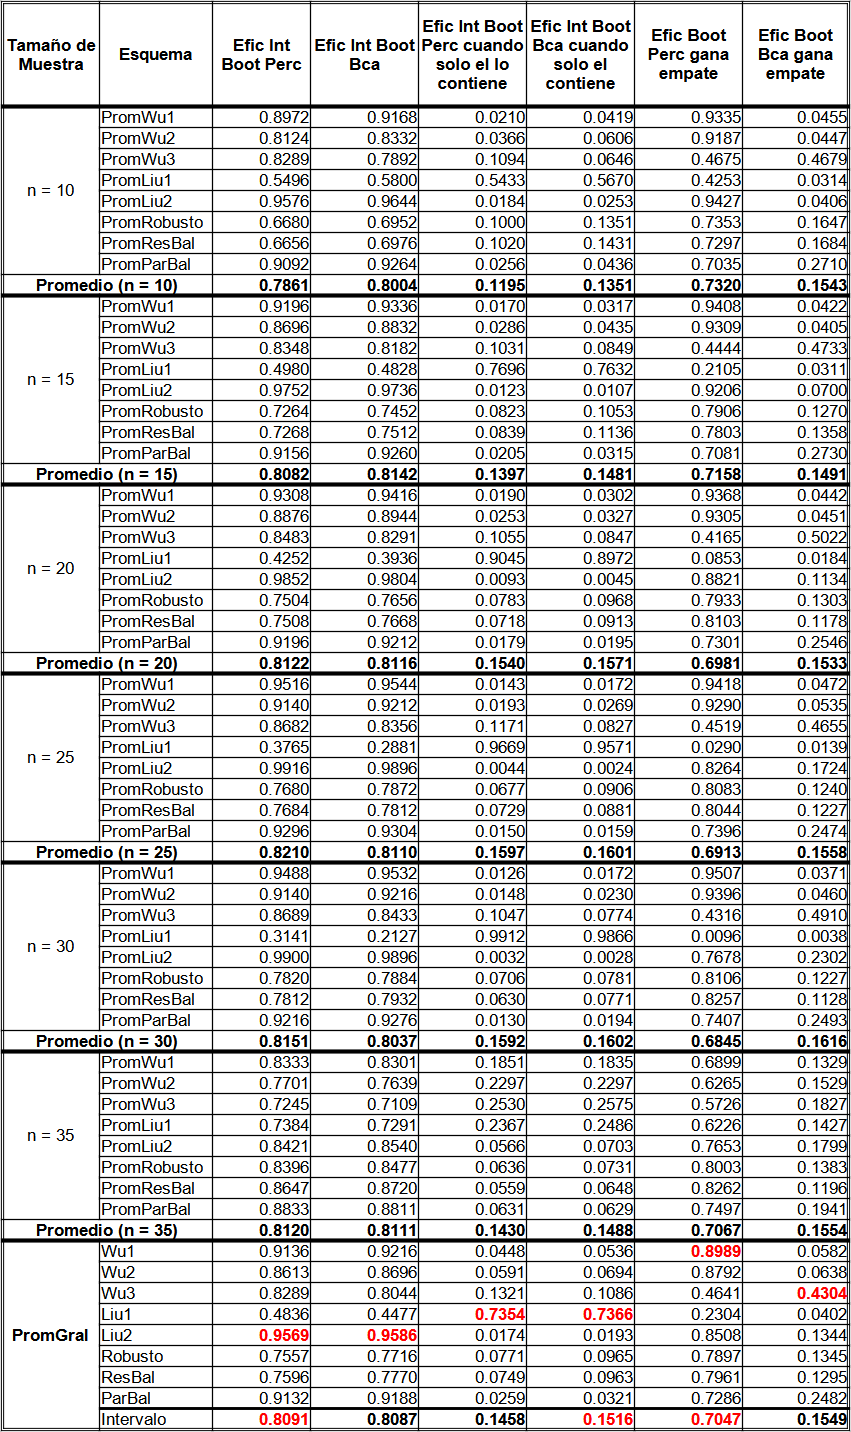
\includegraphics[width=0.55\linewidth]{img/EP_NVC_Efic_Boots.png} 
	\caption{Eficiencia promedio de los intervalos Bootstrap por tamaño de muestra y esquema de remuestreos para el caso EP-NVC.} 
	\label{fig:EP_NVC_Boots}
\end{figure}

\FloatBarrier

\subsection{Eficiencia de los esquemas para el caso EP-NVC}
Con base en un $95\%$ de eficacia, se identifican en color rojo las e cacias
menores a este porcentaje con la nalidad de observar alguna relacion.
\begin{figure}[H] 
	\centering 
	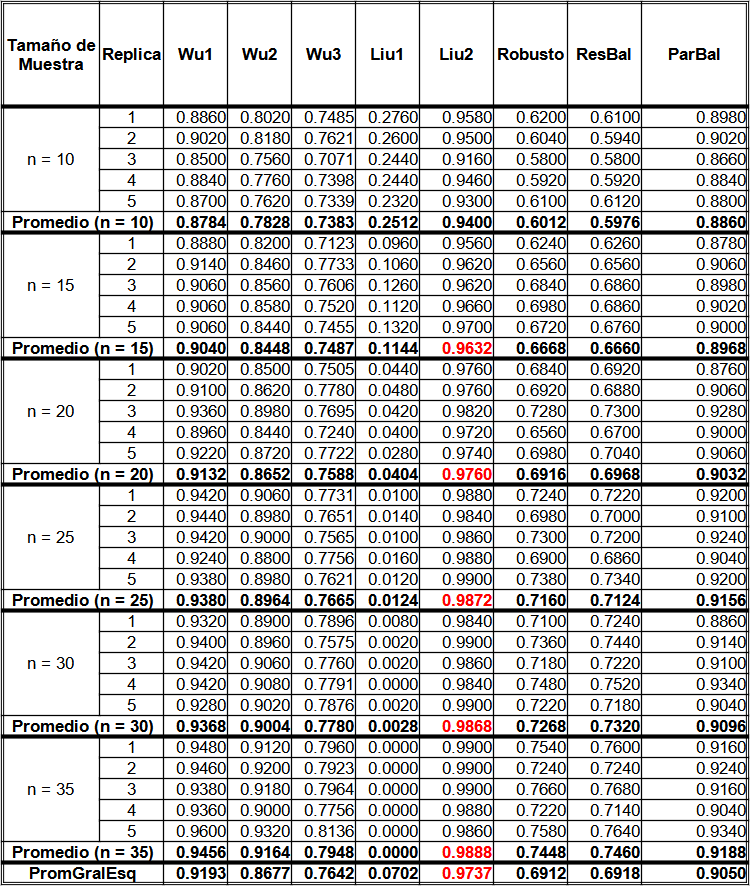
\includegraphics[width=0.70\linewidth]{img/EP_NVC_Efic_Esq.png} 
	\caption{Eficiencia promedio de los esquemas por tamaño de muestra y esquema de remuestreos para el caso EP-NVC.} 
	\label{fig:EP_NVC_Esq}
\end{figure}

\FloatBarrier
